\documentclass{beamer}
\usetheme{default}

\title{Kelompok 5 : Space-Based Architecture}
\subtitle{Mata Kuliah Software Achitecture\\Pradita University}
\author{David Eri Nugroho, Khalid Husein, Ezra Christoper Kid Manopo}
\date{1 April 2023}
\begin{document}
	
	\begin{frame}[plain]
		\maketitle
	\end{frame}
	
	\begin{frame}{Latar Belakang}
		\begin{itemize}
			\item Asal mula terciptanya Space-Based Architecture ini dikarenakan adanya kondisi Triangle-Shaped.
			\item Triangle-Shaped merupakan suatu kondisi ketika kita melakukan scalability dengan cara menambah jumlah aplikasi, server, API, database, ataupun aplikasi lain untuk mengatasi kelambatan di sistem kita.
		\end{itemize}
	\end{frame}
	
	\begin{frame}{Space-Based}
		\begin{itemize}
			\item Space-Based Architecture adalah pendekatan untuk sistem komputasi terdistribusi di mana berbagai komponen berinteraksi satu sama lain dengan bertukar tupel atau entri melalui satu atau lebih ruang bersama.
			\item Space-Based Architecture dirancang khusus untuk mengatasi dan memecahkan masalah skalabilitas yang ekstrem dan konkurensi.
			\item Pola ini juga berguna untuk aplikasi yang volume penggunanya tidak dapat diprediksi.
			\item Pola ini dinamakan berdasar pada konsep tuple space dimana menggunakan shared memory yang terdistribusi.
		\end{itemize}
	\end{frame}

	\begin{frame}{Topology}
		\centering
		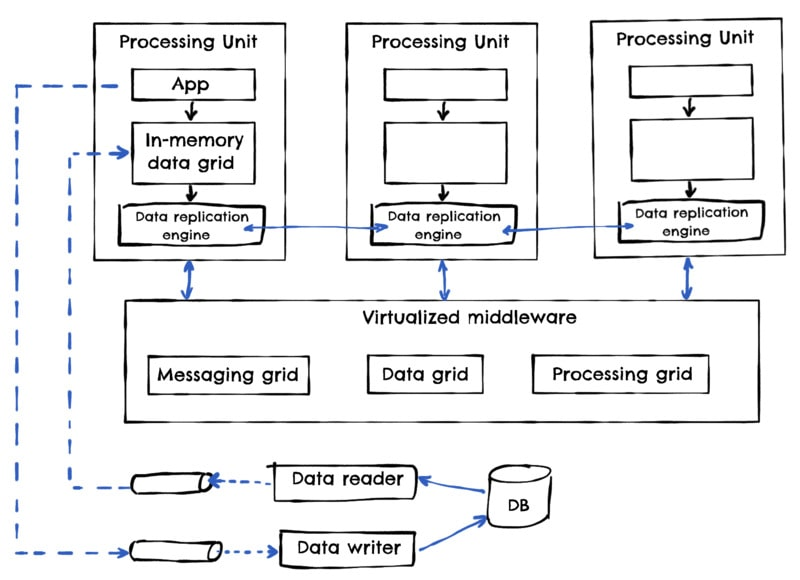
\includegraphics[scale=0.4]{../Downloads/Space-Based Achitecture Topology Vertsiya 1}
	\end{frame}

	\begin{frame}{Sejarah}
		\begin{itemize}
			\item Space-based architecture (SBA) awalnya ditemukan dan dikembangkan di Microsoft pada tahun 1997–98.
			\item Secara internal di Microsoft dikenal sebagai Youkon Distributed Caching platform (YDC).
			\item Proyek web besar pertama berdasarkan itu adalah MSN Live Search (dirilis pada September 1999) dan kemudian penyimpanan data pemasaran Pelanggan MSN (DB dalam memori multi-terabyte yang dibagikan oleh semua situs MSN) serta sejumlah situs MSN lainnya yang dirilis pada akhir 1990-an dan awal 2000-an.
		\end{itemize}
	\end{frame}
	
	\begin{frame}{Kelebihan}
		\begin{itemize}
			\item Merespons dengan cepat terhadap lingkungan yang terus berubah.
			\item Meskipun arsitektur berbasis ruang umumnya tidak dipisahkan dan didistribusikan, mereka dinamis, dan alat berbasis cloud yang canggih memungkinkan aplikasi untuk dengan mudah "didorong" ke server, menyederhanakan penerapan.
			\item Performa tinggi dicapai melalui akses data dalam memori dan mekanisme caching yang dibangun ke dalam pola ini.
			\item Skalabilitas tinggi berasal dari fakta bahwa ada sedikit atau tidak ada ketergantungan pada database terpusat, oleh karena itu pada dasarnya menghilangkan hambatan yang membatasi ini dari persamaan skalabilitas.
		\end{itemize}
	\end{frame}
	
	\begin{frame}{Kekurangan}
		\begin{itemize}
			\item Mencapai beban pengguna yang sangat tinggi dalam lingkungan pengujian adalah hal yang mahal dan memakan waktu, sehingga sulit untuk menguji aspek skalabilitas aplikasi.
			\item Caching yang canggih dan produk grid data dalam memori membuat pola ini relatif kompleks untuk dikembangkan, sebagian besar karena kurangnya pemahaman tentang alat dan produk yang digunakan untuk membuat jenis arsitektur ini. Selain itu, perhatian khusus harus diberikan saat mengembangkan jenis arsitektur ini untuk memastikan tidak ada kode sumber yang memengaruhi kinerja dan skalabilitas.
		\end{itemize}
	\end{frame}
	
	\begin{frame}{Implementasi}
		\begin{itemize}
			\item E-commerce
			\item Permainan online
			\item Sistem sensor jaringan
			\item Sistem analisis data
			\item Aplikasi internet of things
		\end{itemize}
	\end{frame}
	
\end{document}